%! Author = itgramic
%! Date = 29.09.23

% Preamble
\chapter{Abgrenzungen}
Im Kantonsspital Graubünden sind bereits einige Systeme im Einsatz, die gegeben sind.
%\begin{longtable}{@{}lll@{}}
%\toprule
%\textbf{System}                            & \textbf{Produkt}                       & \textbf{Beschreibung}                                                                                    \\* \midrule
%\endfirsthead
%%
%\endhead
%%
%\bottomrule
%\endfoot
%%
%\endlastfoot
%%
%Storage                                    & HPE 3PAR 8450 SAN Storage System       &                                                                                                          \\
%Virtualisierungsplattform                  & VMware® vSphere®                       &                                                                                                          \\
%Primäres Backupsystem                      & VEEAM Backup System                    &                                                                                                          \\
%provisioning / lifecycle management system & Foremann                               & Ist zurzeit nur für Linux angedacht                                                                                                         \\
%Primäre Linux Distribution                 & Debian                                 & RedHat Enterprise Linux oder Oracle Linux wird nur eingesetzt, wenn es nicht anders möglich ist          \\
%Primäres Monitoring System                 & Paessler Router Traffic Grapher (PRTG) & Die Netzwerktechnik nutzt Zabbix                                                                         \\
%Container-Plattform                        & Kubernetes                             &                                                                                                          \\
%Infrastructure as code (Iac) System        & Ansible und Terraform                  & Ansible wird von Foremann verwendet, Terraform wird für die Steuerung der Kubernetes-Plattform verwendet \\
%Usermanagement                             & Microsoft Active Directory             &                                                                                                          \\* \bottomrule
%\caption{Gegebene Systeme}
%\label{gegebene_systeme}
%\end{longtable}
\begin{landscape}
\begin{table}[]
\resizebox{\columnwidth}{!}{%
\begin{tabular}{lll}
\hline
\textbf{}                                 & \textbf{Produkt}                                                                            & \textbf{Beschreibung}                                                                                                                                 \\ \hline
Storage                                   & HPE 3PAR 8450 \Gls{SAN} Storage System                                                            &                                                                                                                                                       \\
Virtualisierungsplattform                 & VMware® vSphere®                                                                            &                                                                                                                                                       \\
Primäres Backupsystem                     & VEEAM Backup System                                                                         &                                                                                                                                                       \\
Provisioning / lifecycle management system & \Gls{Foreman}                                                                                     & Ist zurzeit nur für Linux angedacht                                                                                                                   \\
Primäre Linux Distribution                & \Gls{Debian}                                                                                      &                                                                                                                                                       \\
Sekundäre Linux Distributionen            & \begin{tabular}[c]{@{}l@{}}\Gls{Rocky Linux}\\ \Gls{Oracle Linux}\\ RedHat Enterprise Linux (\Gls{RHEL})\end{tabular} & \begin{tabular}[c]{@{}l@{}}RedHat Enterprise Linux (\Gls{RHEL}), \Gls{Rocky Linux} oder \Gls{Oracle Linux} wird nur eingesetzt,\\ wenn es nicht anders möglich ist\end{tabular} \\
Primäres Monitoring System                & Paessler Router Traffic Grapher (\Gls{PRTG})                                                      & Monitoring System für alle ausser dem Netzwerkbereich                                                                                                 \\
Sekundäres Monitoring System              & \Gls{Zabbix}                                                                                      & Wird nur vom Netzwerkbereich verwendet                                                                                                                \\
Container-Plattform                       & \Gls{Kubernetes}                                                                                  &                                                                                                                                                       \\
Infrastructure as code (Iac) System       & \Gls{Ansible} und \Gls{Terraform}                                                                       & \begin{tabular}[c]{@{}l@{}}\Gls{Ansible} wird von \Gls{Foreman} verwendet, \Gls{Terraform} wird für die Steuerung der \\ \Gls{Kubernetes}-Plattform verwendet\end{tabular}   \\
Logplattform / \Gls{SIEM} System                &                                                                                             & \begin{tabular}[c]{@{}l@{}}Wird neu Ausgeschrieben.\\ Produkt zurzeit nicht definiert\end{tabular}                                                    \\
Usermanagement                            & Microsoft Active Directory                                                                  &                                                                                                                                                       \\ \hline
\end{tabular}%
}
\caption{Gegebene Systeme}
\label{tab:gegebene_systeme}
\end{table}
\end{landscape}

Daraus ergeben sich nach nach Züst, Troxler 2002\cite{EDGTQIKU} folgende Abgrenzungen:
\begin{figure}[H]
    \centering
    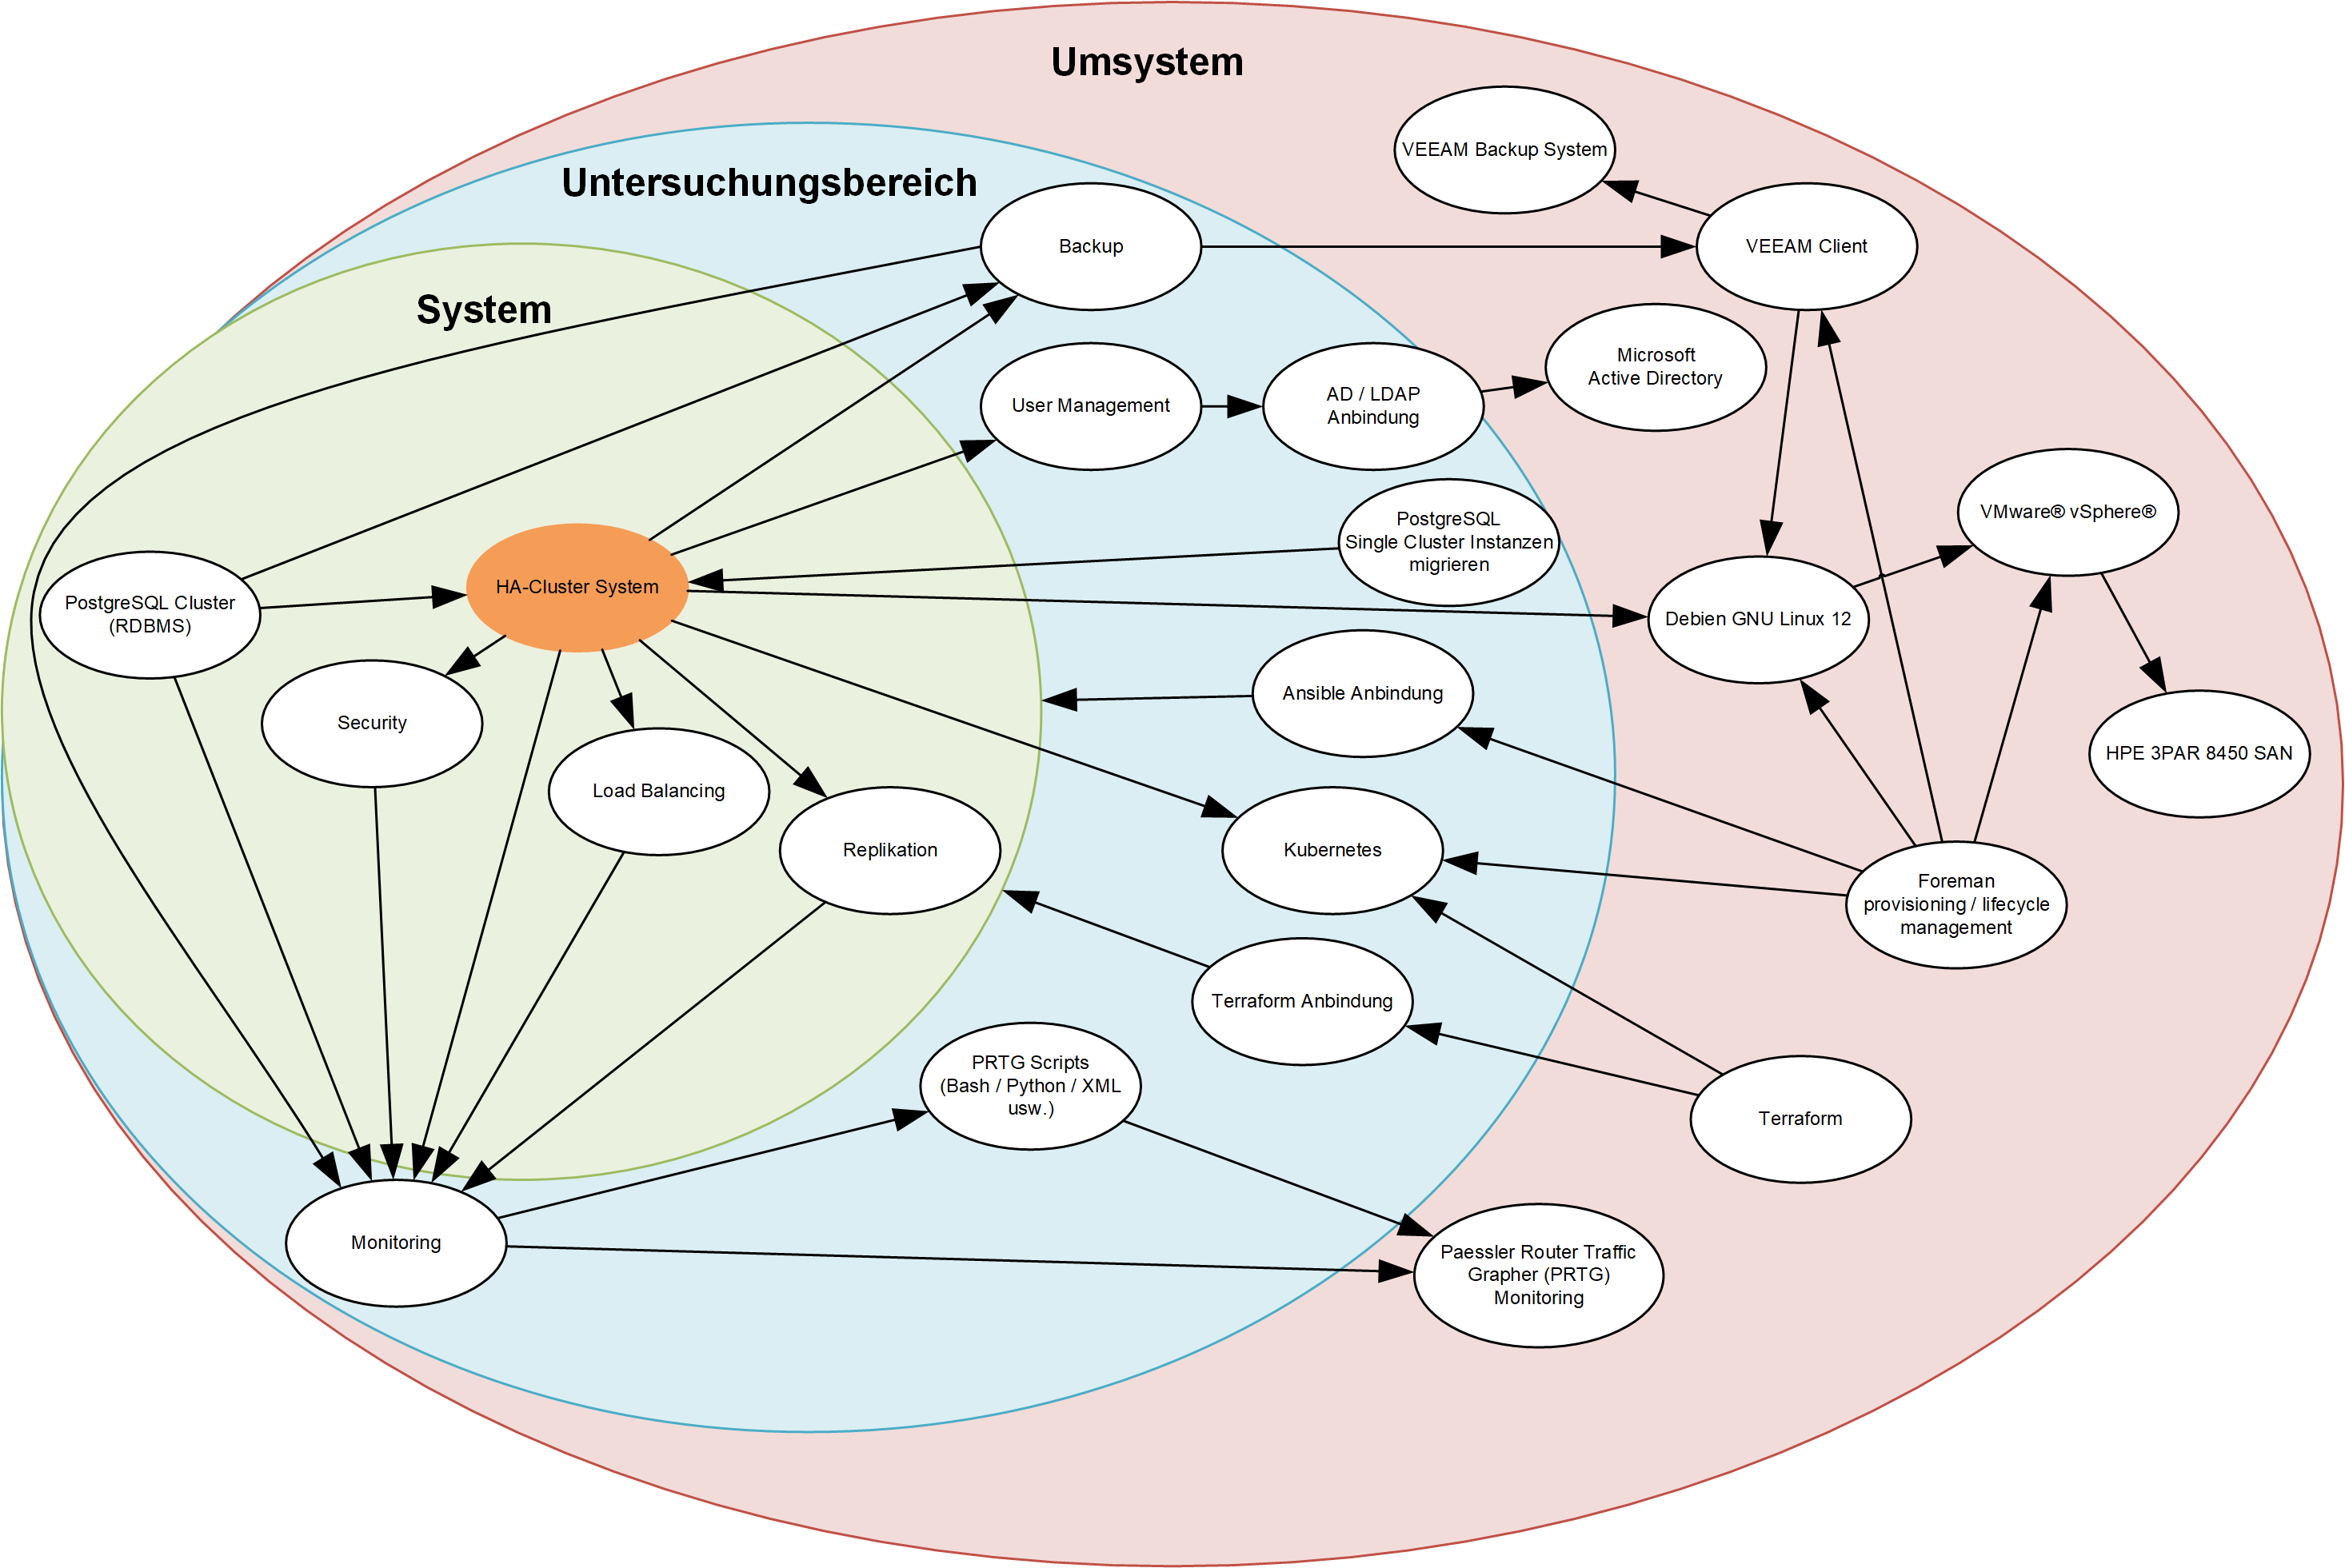
\includegraphics[width=1\linewidth]{source/delimitations/systemabgrenzungen}
    \caption{Systemabgrenzung}
    \label{fig:systemabgrenzungen}
\end{figure}


